\documentclass{article}

\usepackage{polski}
\usepackage{graphicx}
\usepackage{amsmath}
\usepackage{mathtools}
\usepackage{adjustbox}
\usepackage[margin=1in, bmargin=1in, tmargin=0.6in]{geometry}

\author{Paweł Wilkosz}
\title{ON, lista 3 - sprawozdanie}

\begin{document}
\maketitle

\section{Wstęp}
Celem listy jest zbadanie dokładności i efektywności przybliżeń funkcji przy pomocy interpolacji wielomianowej.
Wykorzystanie tej metody pozwala na oszacowanie wartości funkcji, gdy znamy jej wartości tylko w wybranych punktach.

\section{Algorytmy}

\subsection{Ilorazy różnicowe}

W celu wyznaczenia postaci Newtona wielomianu interpolacyjnego należy obliczyć ilorazy różnicowe.

Iloraz różnicowy $k$-tego rzędu zadany jest poniższą zależnością rekurencyjną:

$$
\begin{aligned}
&f[x_0,x_1, \ldots, x_k] = \frac{f[x_1,x_2, \ldots, x_k] - f[x_0, x_1, \ldots, x_{k-1}]}{x_k - x_0}\\
&f[x_0] = f(x_0)\\
&f[x_0,x_1] = \frac{f(x_1) - f(x_0)}{x_1 - x_0}\\
\end{aligned}
$$

Znając węzły $x_k$ i wartości funkcji $f(x_k)$ (czyli również ilorazy $f[x_k]$ zerowego rzędu) można za pomocą tego wzoru utworzyć macierz ilorazów różnicowych wyższych rzędów.
Zapisywanie całej macierzy w pamięci jest jednak nieoptymalne.
Do reprezentacji macierzy ilorazów różnicowych wystarczy użyć jednowymiarowej tablicy $t$.
Początkowymi wartościami zmiennych $t_i$ są odpowiadające im $f[t_i]$, czyli każde $t_i$ obliczane jest ze wzoru:
$$t_i = \frac{t_i-t_{i-1}}{x_i-x_{i-j}}, $$	
gdzie $j$ oznacza numer kolumny w macierzy.
Każda kolejna wartość uaktualniana jest kolumnami, zaś wewnątrz każdej kolumny - z dołu do góry.
Dzięki takiej kolejności obliczeń tablica $t$ zawiera w każdej chwili ilorazy, które będą potrzebne w kolejnych krokach algorytmu.

\subsection{Algorytm Hornera}

Obliczenie ilorazów różnicowych pozwala nam wyznaczyć wilomian interpolacyjny Newtona zadany wzorem
$$
N_n(x) = \sum_{i=0}^k c_i \prod_{j=0}^{i-1}(x-x_j)
$$
gdzie $c_i$ jest ilorazem różnicowym stopnia $i$, zaś $x_j$ - węzłem interpolacji.
Korzystamy z postaci Newtona, która pomimo bardziej skomplikowanej implementacji jest lepiej uwarunkowana numerycznie niż postać LaGrange'a.

W celu obliczenia wartości wielomianu w danym punkcie można zastosować uogólniony algorytm Hornera.
Zasadę jego działania można przedstawić następującym wzorem:
$$
\begin{aligned}
	&w_n(x) := f[x_0, x_1, \ldots, x_n]&\\
	&w_k(x) := w_{k+1}(x-x_k)+ f[x_0, x_1, \ldots, x_k]	\quad(k=n-1, n-2, \ldots, 0)&\\
	&N_n(x) = w_0(x)
\end{aligned}
$$

Zależność ta pozwala wyznaczyć wartość wielomianu w punkcie w czasie liniowym.

\subsection{Postać naturalna}
Wielomianem stopnia $n$ zmiennej $x$ w postaci naturalnej jest wyrażenie postaci
$$
\sum_{i=0}^{n} a_ix^i
$$

W celu znalezienia współczynników wielomianu interpolacyjnego w postaci naturalnej jako punkt wyjścia zastosowano uogólniony algorytm Hornera pokazany w poprzedniej sekcji.
W wielomianie interpolacyjnym $n$-tego stopnia współczynnik $a_n$ przy najwyższej potędze $x$ jest równy $c_n$.
Z tego faktu wynika także, że  $w_n$ z uogólnionego algorytmu Hornera jest również równy $a_n$.
Posiadając $a_n$ = $w_n$ w kolejnych krokach algorytmu tworzone są wartości $a_i$ bazujące na współczynnikach $a_{i+1}$.
Aby znaleźć zależności między kolejnymi $a_i$ algorytm iteruje po wszystkich $w_i$ od $i$ równego $n$ do $0$, tak zmieniając tworzone współczynniki postaci naturalnej, żeby dla każdego $w_i$ doprowadzić w danym momencie do postaci naturalnej.

\subsection{Wykres funkcji i wielomianu interpolowanego}

W celu wizualizacji działania powyższych algorytmów użyjemy funkcji \texttt{rysujNnfx} przyjmującej anonimową funkcję, przedział oraz stopień wielomianu interpolacyjnego.
Następnie rysuje wykres funkcji oraz wielomianu wyznaczonego z równoodległych węzłów za pomocą wcześniej zaimplementowanych funkcji \texttt{ilorazyRoznicowe} i \texttt{warNewton}.


\section{Eksperymenty}

Wszystkie poniższe testy funkcji \texttt{rysujNnfx} zostały przeprowadzone dla $n \in \{5,10,15\}$.

\subsection{Przypadki optymistyczne}

Badamy funkcje $f(x) = e^x$ na przedziale $[0,1]$ i $f(x) = |x|$ na $[-1,1]$.
Wygenerowane wykresy widoczne są na rysunkach \ref{5a} i \ref{5b}.

Można zaobserwować, że zaimplementowane metody interpolacji dają poprawne wyniki już dla najniższego testowanego stopnia wielomianu ($5$).

\begin{figure}
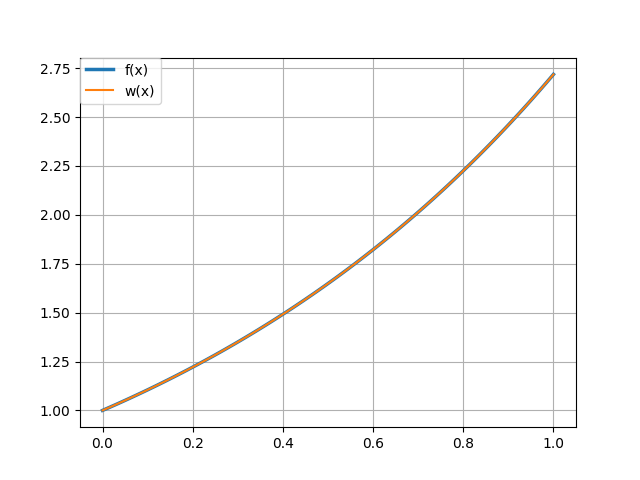
\includegraphics[width=0.3\textwidth]{plots/5a_5.png}
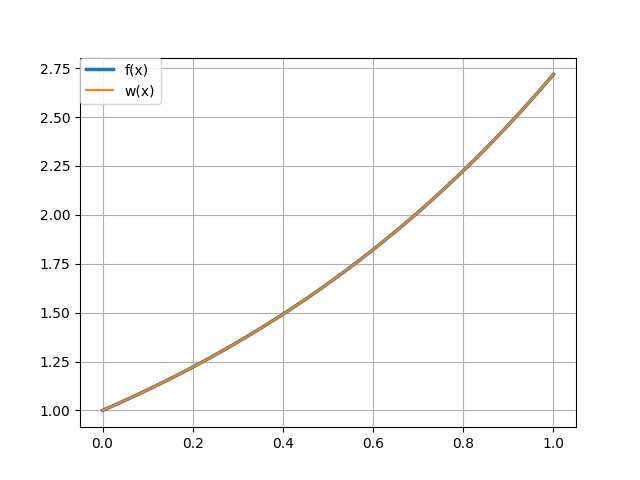
\includegraphics[width=0.3\textwidth]{plots/5a_10.png}
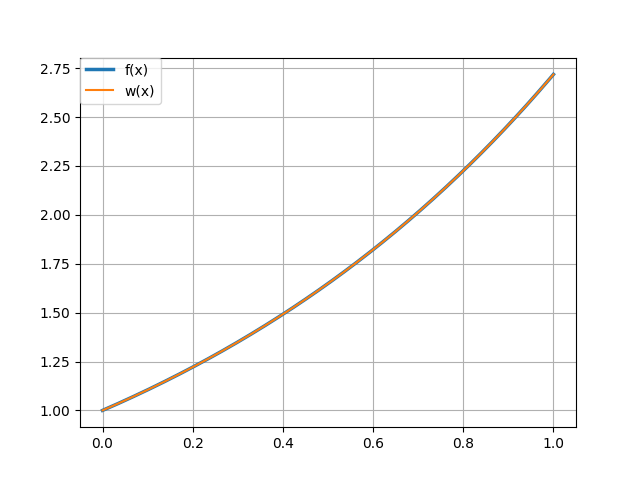
\includegraphics[width=0.3\textwidth]{plots/5a_15.png}
\caption{Wykresy funkcji i wielomianu interpolującego dla $f(x) = e^x$ na przedziale $[0,1]$ dla $n=5,10,15$}
\label{5a}
\end{figure}

\begin{figure}
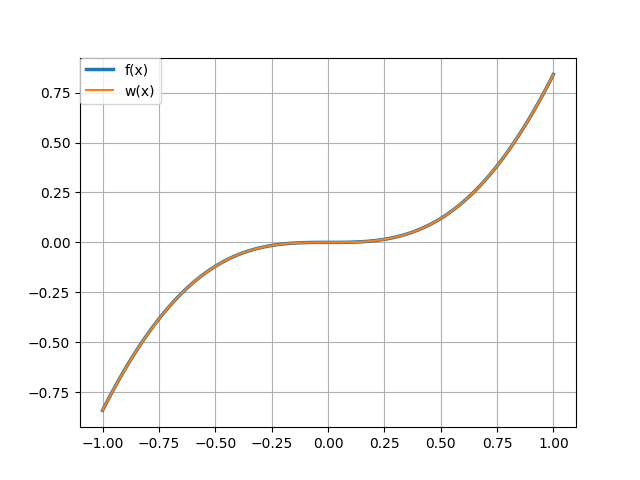
\includegraphics[width=0.3\textwidth]{plots/5b_5.png}
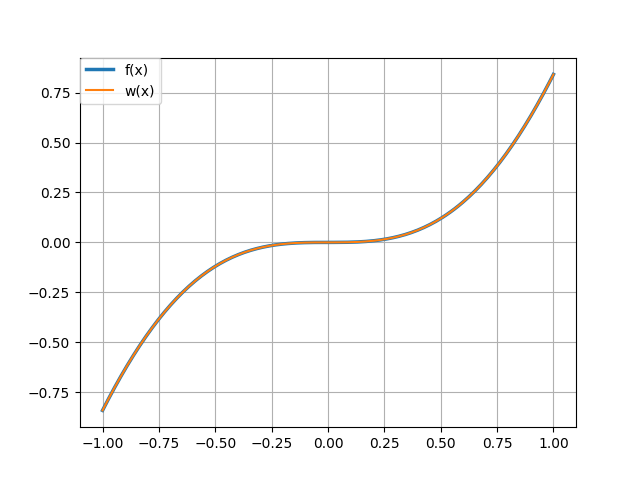
\includegraphics[width=0.3\textwidth]{plots/5b_10.png}
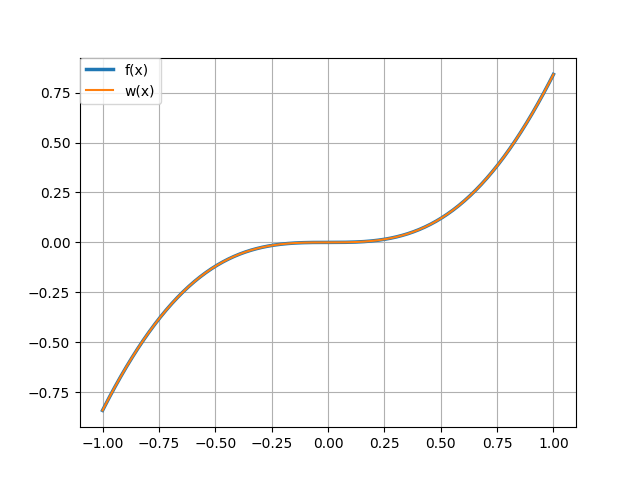
\includegraphics[width=0.3\textwidth]{plots/5b_15.png}
\caption{Wykresy funkcji i wielomianu interpolującego dla $f(x) = x^2\sin x$ na przedziale $[-1,1]$ dla $n=5,10,15$}
\label{5b}
\end{figure}

\subsection{Przypadki pesymistyczne}

Badane metody są jednak podatne na błędy.
Dobrze widoczne jest to na przykładzie funkcji $f(x)=|x|$ na przedziale $[0,1]$ (rysunek \ref{6a}) oraz $f(x) = \frac{1}{1+x^2}$ na $[-5,5]$ (rysunek \ref{6b}).

Pierwszy przypadek pozwala zaobserwować, że wzrost stopnia wielomianu może paradoksalnie powodować mniejszą dokładność.
Można zauważyć, że w wypadku wielomianów wyższego stopnia osiągamy dokładniejsze wartości w okolicach zera, jednak dla argumentów bliższych krańcom przedziału występują duże wahania wartości.

W drugim wypadku wyżej wspomniane wahania są jeszcze bardziej widoczne.

Oscylacje są spowodowane charakterystyką badanych funkcji i są nie do uniknięcia w wypadku stosowania równoodległych węzłów.
Jedynym sposobem na zwiększenie dokładności interpolacji jest zagęszczenie węzłów w problematycznych przedziałach.


\begin{figure}
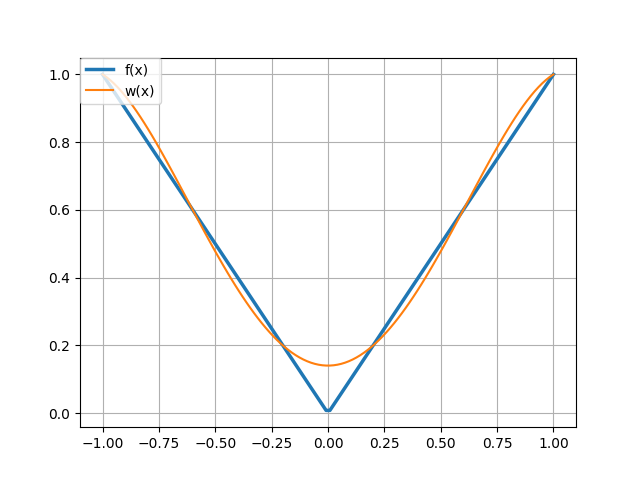
\includegraphics[width=0.3\textwidth]{plots/6a_5.png}
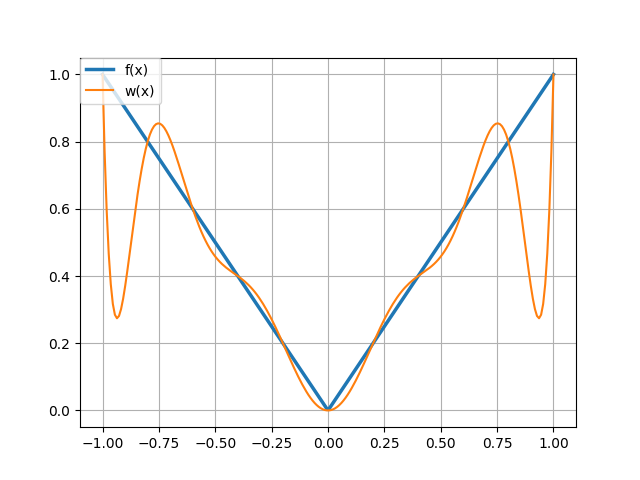
\includegraphics[width=0.3\textwidth]{plots/6a_10.png}
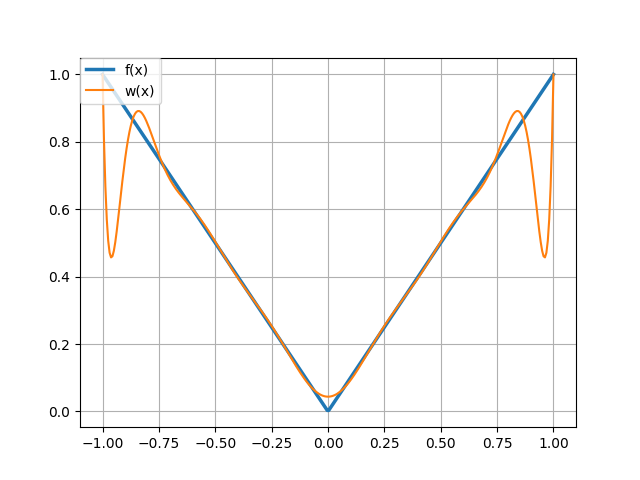
\includegraphics[width=0.3\textwidth]{plots/6a_15.png}
\caption{Wykresy funkcji i wielomianu interpolującego dla $f(x) = |x|$ na przedziale $[-1,1]$ dla $n=5,10,15$}
\label{6a}
\end{figure}


\begin{figure}
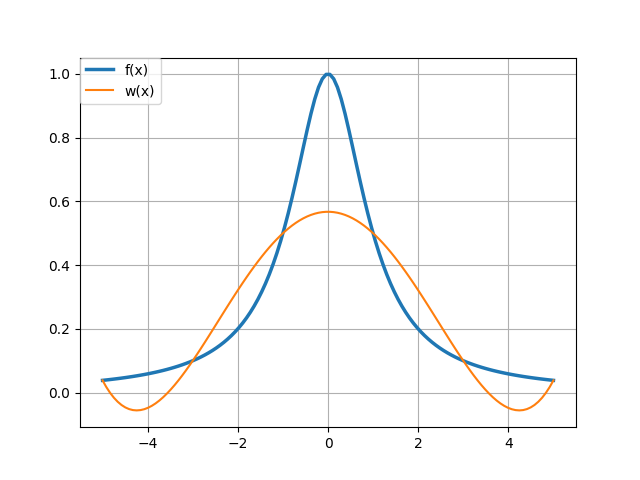
\includegraphics[width=0.3\textwidth]{plots/6b_5.png}
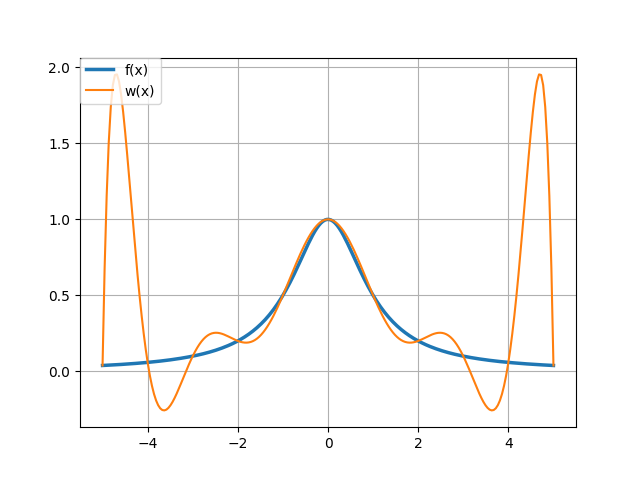
\includegraphics[width=0.3\textwidth]{plots/6b_10.png}
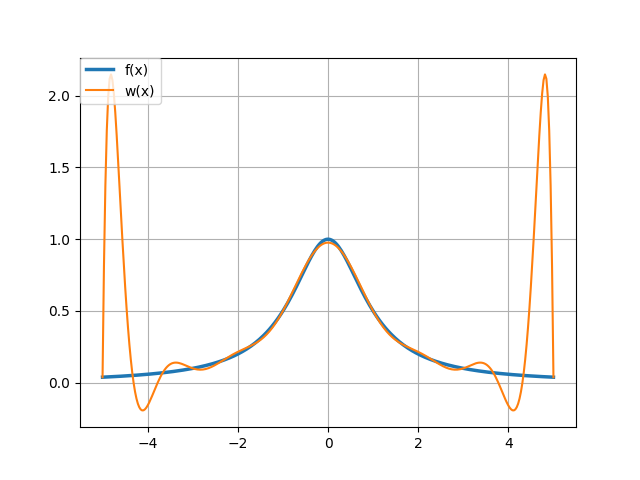
\includegraphics[width=0.3\textwidth]{plots/6b_15.png}
\caption{Wykresy funkcji i wielomianu interpolującego dla $f(x) = \frac{1}{1+x^2}$ na przedziale $[-5,5]$ dla $n=5,10,15$}
\label{6b}
\end{figure}

\section{Wnioski}

Interpolacja wielomianu to efektywna metoda przybliżenia funkcji, gdy znamy tylko część jej wartości.
Powyższe eksperymenty udowadniają jednak, że istnieją funkcje, które, w celu poprawnej interpolacji, wymagają specyficznego rozmieszczenia węzłów.
Powoduje to, że w przypadkach gdy mamy szczątkowe dane, interpolacja nie może być jedyną metodą szacowania przebiegu funkcji.



\end{document}